\documentclass{article}

% Language setting
% Replace `english' with e.g. `spanish' to change the document language
\usepackage{biblatex} %Imports biblatex package
\addbibresource{refs.bib}
\usepackage[english]{babel}
\usepackage{array}
\usepackage{amsmath}
\usepackage{pythonhighlight}
\usepackage{multirow}
\newcolumntype{P}[1]{>{\centering\arraybackslash}p{#1}}
\newcolumntype{M}[1]{>{\centering\arraybackslash}m{#1}}

% Set page size and margins
% Replace `letterpaper' with `a4paper' for UK/EU standard size
\usepackage[letterpaper,top=2cm,bottom=2cm,left=3cm,right=3cm,marginparwidth=1.75cm]{geometry}

\usepackage{amsmath}
\usepackage{graphicx}
\usepackage[colorlinks=true, allcolors=blue]{hyperref}
\usepackage{setspace}
\usepackage{booktabs}
\usepackage[T1]{fontenc}
\usepackage{longtable}
\doublespacing

\begin{document}
\begin{titlepage}

\centering
\scshape
\vspace{\baselineskip}

%
\rule{\textwidth}{1.6pt}\vspace*{-\baselineskip}\vspace*{2pt}
\rule{\textwidth}{0.4pt}

{\Huge \textbf{\textsc{ Hardness and Compression \\
\vspace{15pt}}}}

\rule{\textwidth}{0.4pt}\vspace*{-\baselineskip}\vspace{3.2pt}
\rule{\textwidth}{1.6pt}\vspace{6pt}
\centerline{\textit{University of Illinois at Urbana-Champaign}} 
\centerline{\textit{Department of Nuclear, Plasma, and Radiological Engineering}}
\vspace{1.5\baselineskip}


\large \centerline{\textbf{Author:} Nathan Glaser}
\large \centerline{\textbf{Net-ID:} nglaser3}
\quad

\vfill
\large \centerline{September 18, 2024}
%
\pagenumbering{gobble}
\end{titlepage}

\tableofcontents
\newpage
\pagenumbering{arabic}

\section{Abstract}

Materials, especially in nuclear applications, may encounter extreme external forces. To predict how materials will fare in these scenarios we must have an understanding of its deformation tendencies (plasticity and elasticity) as a function of external load and its resistance to these deformations (hardness). We investigated four materials for their hardness and behaviour under compression: PolyMethyl MethAcrylate (PMMA), 1018 Cold Rolled (CR) steel, 1045 NorMalized (NM) Steel, and 2024 Aluminum alloy. To measure their hardness, we subjected each material (excluding PMMA) to three trials of Rockwell B/C hardness tests. To examine their behaviour under compression we utilized an INSTRON universal testing machine and compressed each of the four materials. Further, we examined the difference in efficacy of three hardness test (Brinnel, Rockwell B/C) on two materials: 2024 Aluminum alloy and 4340 carbon steel. We found that the reliability of the various hardness tests is strongly dependent on the material being tested, and that the conversions from Rockwell B to Brinnel was more inaccurate than from Rockwell C to Brinnel, though it should be noted that the Rockwell C value was outside of the validity range for the conversion, and so we then converted to Vickers instead. 

\newpage
\section{Results}
To begin, we measured the hardness of 2024 aluminum alloy and 4340 carbon steel using Brinnel and Rockwell B/C tests. 20 trials were conducted and tabulated. The statistical information of these trials is presented in Table \ref{table:q1}. Br is Brinnel, and Rb/Rc are Rockwell B/C respectively. Some potential sources of variation for the Brinnel tests are the sheer size of the indenter paired with the number of indents already in the surface and the machine used for testing being more susceptible to user error. The machine utilized was put into place via 'eye-balling', and some tests may have been set up incorrectly. Also, the material surface had 10s of indent already in the surface, and so the likelihood of these indentations affecting nearby material properties is high. The standard deviation of the Rockwell tests was lower, likely due to the lack of, or lower presence of, user error. However, the Rockwell tests were plagued similarly by the quantity of tests the surface was subject to. 

\begin{table}[!hp]
    \def\arraystretch{1.5}
    \centering
    \caption{Hardness Test Statistics for Aluminum Alloy 2024 and Carbon Steel 4340}
    \label{table:q1}
    \begin{tabular}{|c|c|c|c|c|c|c|}
    \toprule
    \hline
    \multicolumn{1}{|c|}{\textbf{Material:}} & \multicolumn{3}{|c|}{\textbf{2024 Aluminum}} & \multicolumn{3}{|c|}{\textbf{4340 Steel}} \\ \hline
    \textbf{Test:} & \textbf{Brinell} & \textbf{Rockwell B} & \textbf{Rockwell C} & \textbf{Brinell} & \textbf{Rockwell B} & \textbf{Rockwell C} \\ 
    \midrule
    \textbf{Mean} & 140.9 & 86.475 & 4.115 & 740.5 & 121.485 & 63.04 \\
    \textbf{Median} & 138. & 86.65 & 5.2 & 731. & 121.55 & 62.85 \\
    \textbf{Std. Dev.} & 6.172 & 2.927 & 3.033 & 38.124 & 0.977 & 1.495 \\
    \hline
\end{tabular}
\end{table} 

To continue, we converted whichever of the Rockwell B/C tests that yielded sensible results to Brinnel utilizing Table 5 and 6 from \cite{manual}. We found the Rockwell B test for 2024 was sensible, and converted to a Brinnel value of 170.95. Further, we found the Rockwell C test for 4340 was sensible, however was outside of the range of validity of the conversion chart presented in Table 6 from \cite{manual}. Thus, we instead converted to Vickers, obtaining a value of 768.1.

Next, we measured the engineering stress and strain of PMMA, 1018CR, 1045NM, and 2024. The engineering stress vs. strain for all of these materials is presented in Fig. \ref{fig:q3all}. The engineering strain is fractional, not percent. 

\begin{figure}[!h!]
    \centering
    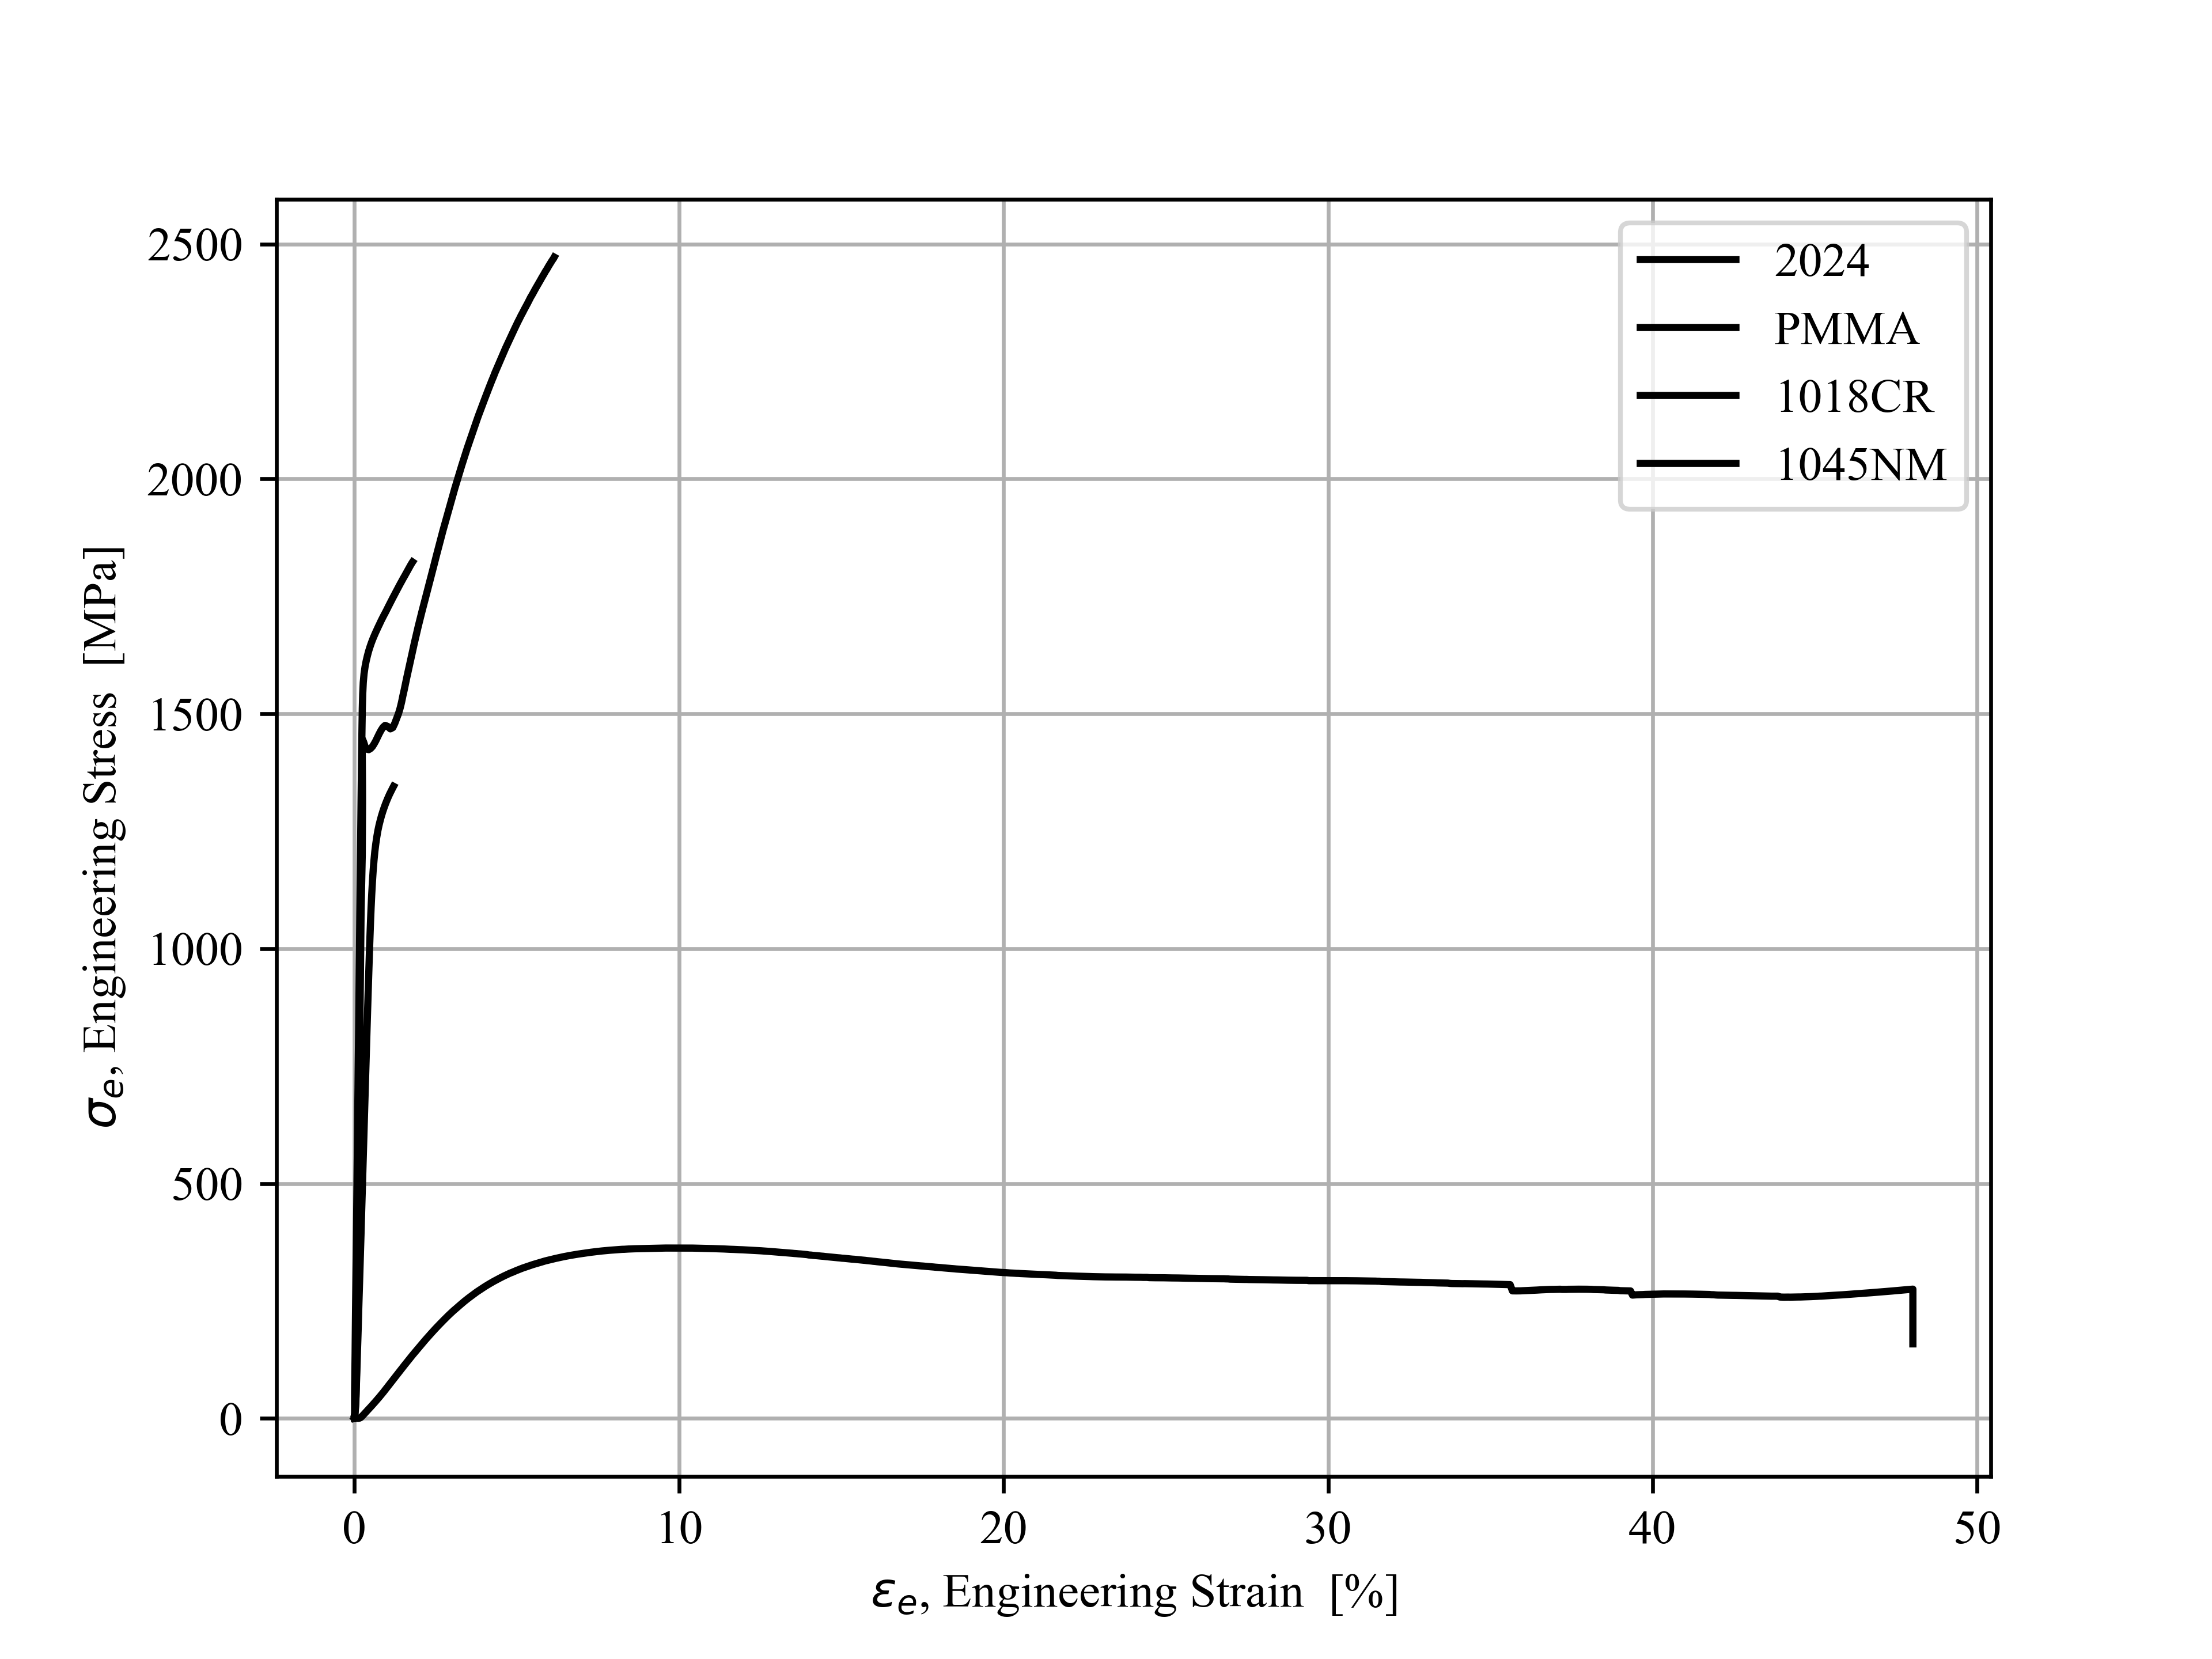
\includegraphics[width=0.7\linewidth]{plots/q3_all.png}
    \caption{$\sigma_e$ against $\epsilon_e$ for all materials}
    \label{fig:q3all}
\end{figure}
\newpage
From Fig. \ref{fig:q3all}, we can deduce information about the relationship between the materials. Most obviously, and unsurprisingly, PMMA plastically deformed the most. This checks out as PMMA is indeed a plastic and the other materials are metals. Next, we can see that both steel alloys were stronger had much higher strength compared to the aluminum alloy (2024). Similarly, the aluminum alloy's elastic modulus is lower than both steels. Again this makes sense as aluminum is a softer metal than steel. Finally, the cold rolled steel alloy, 1018CR, had by far the highest offset strength. 

For specifically the 1045NM steel we also found the true stress and strain. To convert from engineering to true we utilized Eqs. \ref{eq:sigt} and \ref{eq:epst}:

\begin{equation}
    \sigma_t = \sigma_e \left(1+\epsilon_e\right)
    \label{eq:sigt}
\end{equation}
\begin{equation}
    \epsilon_t = ln\left( 1 + \epsilon_e\right)
    \label{eq:epst}
\end{equation}

\noindent
The resulting stress-strain curves are presented in Fig. \ref{fig:evt}:

\begin{figure}[!h!]
    \centering
    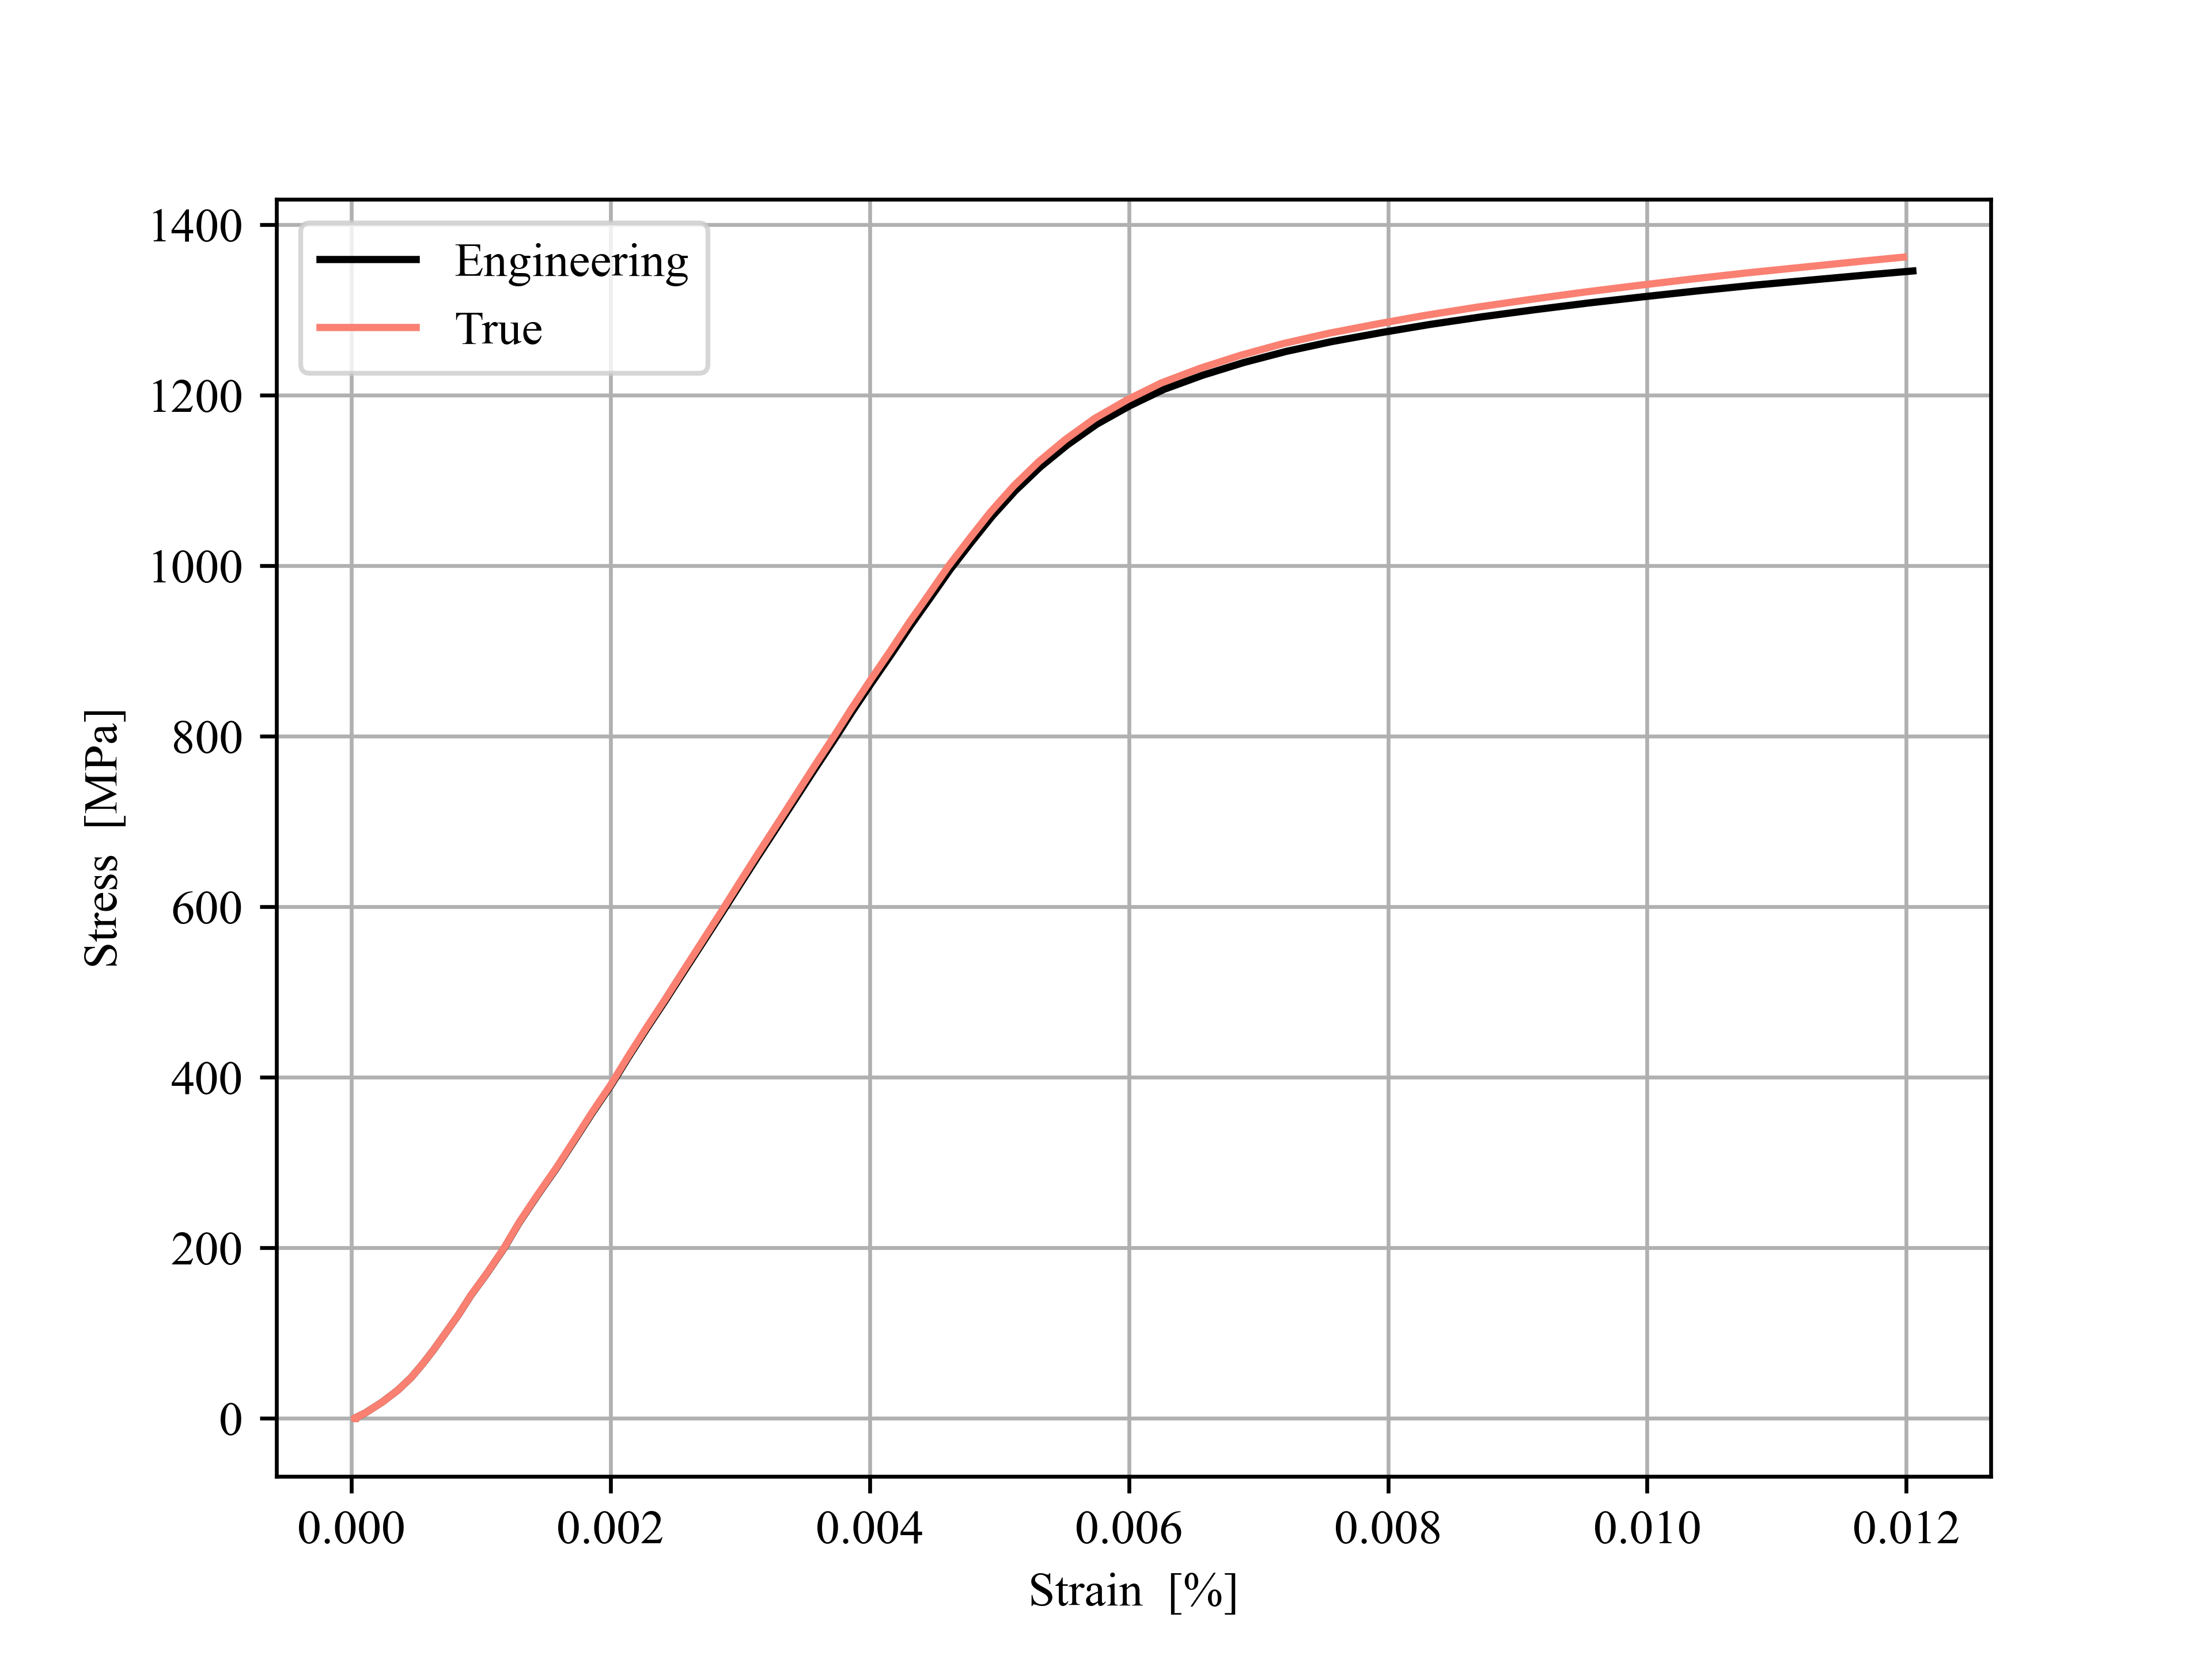
\includegraphics[width=0.7\linewidth]{plots/q3_engvtru.png}
    \caption{True and engineering stress-strain curves for 1045NM steel.}
    \label{fig:evt}
\end{figure}

Finally, from these stress-strain curves we found Young's modulus (elastic modulus), the engineering 0.2 \% offset strength, and the Ultimate Tensile Strength (UTS) for each of the materials. These values are tabulated in Table \ref{tab:q4}.

\begin{table}[!h!]
    \centering
    \def\arraystretch{1.5}
    \caption{Compressive properties of 2024, PMMA, 1018CR, and 1045NM}
    \begin{tabular}{|c|c|c|c|c|}
         \toprule
         \hline
         \textbf{Material} & \textbf{Aluminum 2024} & \textbf{PMMA} & \textbf{1018CR Steel} & \textbf{1045NM Steel}  \\
         \midrule
         \textbf{Elastic Modulus [GPa]} & 73.15001 & 2.64300 & 20.36786 & 229.89836 \\
         \hline
         \textbf{0.2\% Offset [MPa]} & 401.0 & 6.543 & 521.353 & 453.422\\
         \hline
         \textbf{UTS [MPa]} & 428.35061 & 115.49504 & 580.35601 & 786.92962 \\
         \bottomrule
    \end{tabular}
    
    \label{tab:q4}
\end{table}

\newpage
\section{Bibliography}
\printbibliography[heading=none]

\end{document}